\documentclass[a4paper,10pt]{article}
\usepackage[utf8]{inputenc}
\usepackage[T1]{fontenc}
\usepackage[french]{babel}
\usepackage{textcomp}
\usepackage{amsmath,amssymb}
\usepackage{lmodern}
\usepackage{graphicx}
\usepackage[dvipsnames,svgnames]{xcolor}
\usepackage{microtype}
\usepackage{listings}
\usepackage{mathtools}
\lstset{
upquote = true,
columns = flexible,
basicstyle = \ttfamily,
keepspaces=true,
language = python,
backgroundcolor = \color{Navy!10},
keywordstyle = \color{Blue}\bfseries,
numbers=left, numberstyle=\tiny,
tabsize = 4,
}
\usepackage{dashbox}
\usepackage{colortbl}
\newtheorem{theoreme}{Théorème}[section]
\newtheorem{lemme}[theoreme]{Lemme}
\newtheorem{exo}{Exercice}
\newtheorem{remarque}{Remarque}
\newtheorem{corollaire}[theoreme]{Corollaire}
\usepackage{csquotes}
\usepackage[
bibstyle=numeric,
citestyle=numeric-comp,
]{biblatex}
\addbibresource{biblio.bib}
\usepackage{hyperref} 
\hypersetup{colorlinks=true, 
            linkcolor=Black, 
            urlcolor=Navy, 
            breaklinks=true, 
            bookmarks=true, 
            pdfstartview=XYZ
}

\title{\Huge\bfseries\MakeUppercase{Analyse des tris empiriques}}
\author{Charlotte Montanari}

\begin{document}

\maketitle 
\tableofcontents


\section{Introduction}
Pour cet exposé, j'ai décidé de le faire sur les tris empiriques, un cours que nous avons eu l'année dernière avec 
Mr Zanotti \cite{zanotti}.

\section{Le tri par selection}
\subsection{Présentation de l'algorithme}
Le tri par sélection est l'un des tris les plus simples. 
Il s'appuie sur un algorithme auxiliaire de re­cher­che du \textcolor{blue}{minimum} (ou symétriquement 
du \textcolor{blue}{maximum}) dans une liste (supposée non-vide). 
Pour cette recherche, on initialise toujours le minimum (ou le maximum) 
au premier terme de la liste puis on parcourt le reste des termes de la liste en mettant à jour 
la valeur minimale (ou maximale) si le terme courant est plus petit (ou plus grand):
\lstinputlisting{algomin.py}

L'écriture de l'algorithme coule de source, il suffit de répéter la recherche de 
l'indice du minimum (instruction \#5), de faire l'échange (instruction \#6) et de 
recommencer un cran plus loin dans la liste (incrément de l'indice de départ dans la liste, instruction \#7):
\begin{center}
    \lstinputlisting{algotriselection.py}
    Algorithme de tri par sélection\label{algotriselection}
\end{center}

La trace de l'exécution du \textcolor{blue}{TriSelection} \ref{algotriselection} pour la liste L = [3,5,2,1,7,4,6]
ci-dessous permet de comprendre le processus. Chaque ligne représente une étape dans la recherche du minimum, 
il est distingué des autres valeurs par un \textcolor{green}{fond clair}, la valeur à laquelle il est comparé 
est \dashbox{encadrée} et apparaît sur \textcolor{red}{fond rouge} dans le cas où elle est inférieure à la valeur minimale, 
indiquant ainsi qu'il faudra mettre à jour l'indice $i_{min}$. Ces mises à jour ainsi que les {\itshape n} $-$ 1 
échanges réalisés, sont spé­ci­fiés dans la dernière colonne.

\begin{center}
\begin{tabular}{|c|c|c|c|c|c|c|c|c|}
    \hline
    i = & 1 & 2 & 3 & 4 & 5 & 6 & 7 & \\
    \hline
    \#1 & \cellcolor{green}{3} & \dashbox{5} & 2 & 1 & 7 & 4 & 6 & \\
    \hline
    \#2 & \cellcolor{green}{3} & 5 & \cellcolor{red}\dashbox{2} & 1 & 7 & 4 & 6 & $i_{min} \leftarrow 3$\\
    \hline
    \#3 & 3 & 5 & \cellcolor{green}{2} & \cellcolor{red}\dashbox{1} & 7 & 4 & 6 & $i_{min} \leftarrow 4$\\
    \hline
    \#4 & 3 & 5 & 2 & \cellcolor{green}{1} & \dashbox{7} & 4 & 6 & \\
    \hline
    \#5 & 3 & 5 & 2 & \cellcolor{green}{1} & 7 & \dashbox{4} & 6 & \\
    \hline
    \#6 & 3 & 5 & 2 & \cellcolor{green}{1} & 7 & 4 & \dashbox{6} & $L[1] \rightleftarrows L[4]$\\
    \hline
    \#7 & 1 & \cellcolor{green}{5} & \cellcolor{red}\dashbox{2} & 3 & 7 & 4 & 6 & $i_{min} \leftarrow 3$\\
    \hline
    \#8 & 1 & 5 & \cellcolor{green}{2} & \dashbox{3} & 7 & 4 & 6 & \\
    \hline
    \#9 & 1 & 5 & \cellcolor{green}{2} & 3 & \dashbox{7} & 4 & 6 & \\
    \hline
    \#10 & 1 & 5 & \cellcolor{green}{2} & 3 & 7 & \dashbox{4} & 6 & \\
    \hline
    \#11 & 1 & 5 & \cellcolor{green}{2} & 3 & 7 & 4 & \dashbox{6} & $L[2] \rightleftarrows L[3]$\\
    \hline
    \#12 & 1 & 2 & \cellcolor{green}{5} & \cellcolor{red}\dashbox{3} & 7 & 4 & 6 & $i_{min} \leftarrow 4$\\
    \hline
    \#13 & 1 & 2 & 5 & \cellcolor{green}{3} & \dashbox{7} & 4 & 6 & \\
    \hline
    \#14 & 1 & 2 & 5 & \cellcolor{green}{3} & 7 & \dashbox{4} & 6 & \\
    \hline
    \#15 & 1 & 2 & 5 & \cellcolor{green}{3} & 7 & 4 & \dashbox{6} & $L[3] \rightleftarrows L[4]$\\
    \hline
    \#16 & 1 & 2 & 3 & \cellcolor{green}{5} & \dashbox{7} & 4 & 6 & \\
    \hline
    \#17 & 1 & 2 & 3 & \cellcolor{green}{5} & 7 & \cellcolor{red}\dashbox{4} & 6 & $i_{min} \leftarrow 6$\\
    \hline
    \#18 & 1 & 2 & 3 & 5 & 7 & \cellcolor{green}{4} & \dashbox{6} & $L[4] \rightleftarrows L[6]$\\
    \hline
    \#19 & 1 & 2 & 3 & 4 & \cellcolor{green}{7} & \cellcolor{red}\dashbox{5} & 6 & $i_{min} \leftarrow 6$\\
    \hline
    \#20 & 1 & 2 & 3 & 4 & 7 & \cellcolor{green}{5} & \dashbox{6} & $L[5] \rightleftarrows L[6]$\\
    \hline
    \#21 & 1 & 2 & 3 & 4 & 5 & \cellcolor{green}{7} & \cellcolor{red}\dashbox{6} & $i_{min} \leftarrow 7$ $L[6] \rightleftarrows L[7]$\\
    \hline
\end{tabular}
\end{center}
\begin{center}
    Trace de l'exécution de l'algorithme du tri sélection
\end{center}

\begin{exo}
    Trouvez un contre-exemple qui prouve que le tri par sélection n'est pas un tri stable.
\end{exo}

\subsection{Complexité du tri par selection}
Nous allons estimer la complexité de l'algorithme \textcolor{blue}{TriSelection} \ref{algotriselection} 
en évaluant tout d'abord celle de l'al­gor­i­thme \textcolor{blue}{IdxMin}. Elle dépend des indices {\itshape g} et {\itshape d},
le nombre d'opérations est pro­por­tion­nel au nombre de cellules à parcourir dans le liste L, soit 
{\itshape d} $-$ {\itshape g} $+$ 1. Le nombre réel d'opérations à réaliser dépend bien entendu du nombre 
de mises à jour de l'indice du minimum fonction de l'instance considérée, mais le coût unitaire est borné par 
deux constantes donc en $\theta(1)$. Comme l'appel à cet al­go­ri­thme se fait toujours pour la valeur
{\itshape d} $=$ {\itshape n}, on a \[ T_{IdxMin}(n,d) = \theta(n - d + 1) = \theta(n - d). \]
Les deux algorithmes \textcolor{blue}{Echanger} et \textcolor{blue}{IdxMin} ont tous deux un coût qui ne 
dépend que de la taille des don­nées à traiter et pas de la nature des instances de taille {\itshape n},
par conséquent les trois complexités dans le meilleur des cas, le pire des cas et le cas moyen se confondent.
Toutes les instructions hors de la boucle "tant que" de l'algorithme \textcolor{blue}{TriSelection} \ref{algotriselection} 
ont un coût constant $\theta(1)$ et les trois instructions dans la boucle ont pour coûts respectifs
$\theta(n - d)$, $\theta(1)$ et $\theta(1)$, on en déduit la somme:

\begin{align*}
    T(n) & = \theta(1) + \sum_{d=1}^{n-1}(\theta(n - d) + \theta(1) + \theta(1)) \\
         & = \theta(1) + 2(n - 1)\theta(1) + \sum_{d=1}^{n-1}\theta(n - d) \\
         & = \theta(n) + \sum_{k=1}^{n-1}\theta(k) \\
         & = \theta(n) + \theta(\frac{n(n - 1)}{2}) \\
         & = \theta(n^2)
\end{align*}


\section{Le tri par propagation (tri à bulles)}
\subsection{Présentation de l'algorithme}
Le principe du tri par propagation, généralement connu comme le "tri à bulles" est simple lui aussi. 
La mé­ta­pho­re est que le début de la liste symbolise le fond de l'eau et la fin de la liste la surface. 
Chaque nom­bre représente le diamètre d'une bulle et la bulle la plus grosse est celle qui remonte le plus vite 
à la surface (ce qui est conforme à la réalité physique dans une certaine mesure). Plus formellement, 
on parcourt la liste de la gauche vers la droite en échan­geant les termes contigüs L[i] et L[i$+$1] s'ils sont mal rangés, 
c'est-à-dire si L[i$+$1] < L[i] (on "propage la bulle" L[i]). À ce stade, la bulle la plus grosse 
(la plus grande valeur) est au bout de la liste en position {\itshape n}. 

\begin{lemme}
    À l'issu d'un passage sur la liste L, on a l'assertion L(n) = maxL
\end{lemme}

Le terme le plus grand étant à présent placé au bout de la liste, il suffit de recommencer 
le processus de propagation, mais cette fois sur la sous-liste L[1 : {\itshape n}$-$1] con­te­nant les {\itshape n} $-$ 1 
premiers termes de la liste et ainsi de suite en "éliminant" le dernier terme de la liste à chaque passe. 
L'algorithme est constitué d'une boucle principale (ligne \#3) qui fait varier la taille de la zone [1, {\itshape d}]
à parcourir dans la liste L en commençant par la liste entière avec $d \coloneqq \#L$
en appelant à chaque étape l'algorithme de propagation.
\lstinputlisting{triabulle.py}\label{algotriabulle}
\begin{center}
    Algorithme de Tri par propagation
\end{center}

On peut améliorer immédiatement cet algorithme en remarquant que si aucun échange n'a lieu 
lors d'une passe sur la liste c'est qu'elle est triée et qu'il est alors inutile de balayer la liste à nouveau.

\begin{lemme}
    Si aucun échange n'a eu lieu lors d'une passe sur la liste par l'algorithme \textcolor{blue}{Propager} 
    alors la liste est triée.
\end{lemme}

L'algorithme peut alors exploiter cette optimisation à l'aide de la variable booléenne 
continuer ini­tia­li­sée à \textbf{vrai} au départ et mise à jour par l'algorithme \textcolor{blue}{Propager}.
\lstinputlisting{tribulles.py}

La table ci-dessous montre l'évolution de la liste pendant l'exécution de l'algorithme 
\textcolor{blue}{TriBulles} \ref{algotriabulle}. À chaque étape, les deux termes comparés sont matérialisés 
sur un \textcolor{red}{fond rouge} ou \textcolor{green}{fond vert} selon que leurs indices constituent 
une inversion et qu'il faut les échanger ou non. Le terme d'indice est \dashbox{encadré}.

\begin{center}
    \begin{tabular}{|c|c|c|c|c|c|c|c|c|}
        \hline
        i = & 1 & 2 & 3 & 4 & 5 & 6 & 7 & \\
        \hline
        \#1 & \cellcolor{green}\dashbox{3} & \cellcolor{green}{5} & 2 & 1 & 7 & 4 & 6 & \\
        \hline
        \#2 & 3 & \cellcolor{red}\dashbox{5} & \cellcolor{red}{2} & 1 & 7 & 4 & 6 & $\rightleftarrows$\\
        \hline
        \#3 & 3 & 2 & \cellcolor{red}\dashbox{5} & \cellcolor{red}{1} & 7 & 4 & 6 & $\rightleftarrows$\\
        \hline
        \#4 & 3 & 2 & 1 & \cellcolor{green}\dashbox{5} & \cellcolor{green}{7} & 4 & 6 & \\
        \hline
        \#5 & 3 & 2 & 1 & 5 & \cellcolor{red}\dashbox{7} & \cellcolor{red}{4} & 6 & $\rightleftarrows$\\
        \hline
        \#6 & 3 & 2 & 1 & 5 & 4 & \cellcolor{red}\dashbox{7} & \cellcolor{red}{6} & $\rightleftarrows$\\
        \hline
        \#7 & \cellcolor{red}\dashbox{3} & \cellcolor{red}{2} & 1 & 5 & 4 & 6 & 7 & $\rightleftarrows$\\
        \hline
        \#8 & 2 & \cellcolor{red}\dashbox{3} & \cellcolor{red}{1} & 5 & 4 & 6 & 7 & $\rightleftarrows$\\
        \hline
        \#9 & 2 & 1 & \cellcolor{green}\dashbox{3} & \cellcolor{green}{5} & 4 & 6 & 7 & \\
        \hline
        \#10 & 2 & 1 & 3 & \cellcolor{red}\dashbox{5} & \cellcolor{red}{4} & 6 & 7 & $\rightleftarrows$\\
        \hline
        \#11 & 2 & 1 & 3 & 4 & \cellcolor{green}\dashbox{5} & \cellcolor{green}{6} & 7 & \\
        \hline
        \#12 & \cellcolor{red}\dashbox{2} & \cellcolor{red}{1} & 3 & 4 & 5 & 6 & 7 & $\rightleftarrows$\\
        \hline
        \#13 & 1 & \cellcolor{green}\dashbox{2} & \cellcolor{green}{3} & 4 & 5 & 6 & 7 & \\
        \hline
        \#14 & 1 & 2 & \cellcolor{green}\dashbox{3} & \cellcolor{green}{4} & 5 & 6 & 7 & \\
        \hline
        \#15 & 1 & 2 & 3 & \cellcolor{green}\dashbox{4} & \cellcolor{green}{5} & 6 & 7 & \\
        \hline
        \#16 & \cellcolor{green}\dashbox{1} & \cellcolor{green}{2} & 3 & 4 & 5 & 6 & 7 & \\
        \hline
        \#17 & 1 & \cellcolor{green}\dashbox{2} & \cellcolor{green}{3} & 4 & 5 & 6 & 7 & \\
        \hline
        \#18 & 1 & 2 & \cellcolor{green}\dashbox{3} & \cellcolor{green}{4} & 5 & 6 & 7 & \\
        \hline
    \end{tabular}
    \end{center}
\begin{center}
    Trace de l'exécution de l'algorithme du tri à bulles
\end{center}


\subsection{Complexité du tri à bulles}
Dans le meilleur des cas, les valeurs sont déjà triées et le premier passage suffit à achever 
la pro­cé­du­re puisque la variable continuer reste fausse car aucun échange n'a eu lieu. On a donc réalisé {\itshape n} $-$ 1
comparaisons entre les termes de la liste et \[ \check{T}(n) = \theta(n). \]

Dans le pire des cas, les valeurs sont triées dans l'ordre inverse et il y a sys­té­ma­ti­que­ment 
une per­mu­ta­tion après chaque comparaison entre deux termes contigüs. La taille de la sous-liste 
à traiter décroit d'une unité à chaque nouveau passage, on retrouve la somme des {\itshape n} $-$ 1
premiers entiers soit \[ \hat{T}(n) = \theta(n^2). \]

Notons que la constante cachée est $\frac{1}{2}$. Le nombre moyen de comparaisons est très difficile à ob­te­nir 
dans la version présentée plus haut et qui arrête le processus de tri si aucun échange n'a eu 
lieu lors de la passe précédente. Sans cette optimisation, on retrouve exactement le même nombre 
de comparaisons que dans le pire des cas. En revanche, le nombre moyen d'échanges est exactement le même 
que pour le tri par insertion que nous allons étudier plus loin.

\begin{remarque}
    Il est tentant d'estimer la complexité d'un algorithme de tri à travers le nombre de transpositions 
    nécessaires pour réordonner les termes de la liste L. C'est (probablement) l'analogie avec le coût physique 
    d'une transposition (intervertir deux cartes dans une main par exemple) qui est plus important qu'une simple 
    comparaison (contrôle visuel) qui nous le suggère. Le fonctionnement du tri à bulles (optimisé) permet de se 
    convaincre que ce serait une erreur. En effet dans le cas où la liste est déjà triée, aucune transposition n'est 
    effectuée et il aura pourtant fallu balayer l'intégralité des termes de la liste pour s'en assurer, 
    le coût est donc bien linéaire et pas nul.
\end{remarque}


\section{Le tri par insertion}
\subsection{Présentation de l'algorithme}
Le tri par insertion est le plus "difficile" des trois. C'est celui que nous utilisons quand nous jouons aux cartes, 
plus précisément pendant la phase où l'on range ses cartes dans l'ordre croissant dans sa main. 
Chaque nouvelle carte est {\itshape insérée} à la bonne position par rapport aux cartes déjà rangées. 
L'insertion se fait en comparant la nouvelle carte avec celles déjà en main de la gauche vers la droite (ou le contraire) 
jusqu'à ce que la bonne position soit trouvée.

Il faut néanmoins adapter ce que nous faisons physiquement avec les modèles de données que nous 
manipulons et respecter les contraintes fixées. Nous voulons réaliser le tri in situ, on ne dispose donc que 
de la liste d'origine L et d'un nombre de variables indépendant de sa taille {\itshape n}.
Il faut donc imaginer que l'on va devoir ranger la i-ème carte L[i] dans la sous-liste L[1 : {\itshape i} $-$ 1]
qui est donc supposée triée (on rappelle que l'intervalle entier [a:b] contient toutes les valeurs entre {\itshape a} et 
{\itshape b} incluses contrairement au Python qui exclut {\itshape b}).

L'insertion d'une carte L[i] dans la main/liste L[1 : {\itshape i} - 1] se fait indifféremment en 
parcourant les cartes dans la main de la gauche vers la droite ou de la droite vers la gauche. 

\lstinputlisting{algoinserer.py}

Comme pour le tri à bulle, on arrête la propagation dès que la carte/bulle est bien placée. 
Il suffit alors d'insérer toutes les cartes dans la main de la deuxième carte (la première l'est déjà) 
jusqu'à la dernière carte pour réaliser ce tri.

\lstinputlisting{algotriinsertion.py}

La trace de l'exécution du TriInsertion pour la liste L = [3,5,2,1,7,4,6] ci-dessous permet de comprendre le processus. 
Chaque ligne de la table représente une étape de l'insertion de la carte. Si la carte elle est à la bonne 
position elle est sur fond clair et si elle doit être déplacée, elle est sur fond fond rouge, la zone qui a 
été balayée pour l'insertion de la carte reste sur fond clair. Les différents échanges $\rightleftarrows$
réalisés entre L[{\itshape j}] et L[{\itshape j} - 1] sont spécifiés dans la dernière colonne.

\begin{center}
    \begin{tabular}{|c|c|c|c|c|c|c|c|c|}
        \hline
        i = & 1 & 2 & 3 & 4 & 5 & 6 & 7 & \\
        \hline
        \#1 & 3 & \cellcolor{green}\dashbox{5} & 2 & 1 & 7 & 4 & 6 & \\
        \hline
        \#2 & 3 & 5 & \cellcolor{red}\dashbox{2} & 1 & 7 & 4 & 6 & $\rightleftarrows$\\
        \hline
        \#3 & 3 & \cellcolor{red}\dashbox{2} & \cellcolor{green}{5} & 1 & 7 & 4 & 6 & $\rightleftarrows$\\
        \hline
        \#4 & \cellcolor{green}\dashbox{2} & \cellcolor{green}{3} & \cellcolor{green}{5} & 1 & 7 & 4 & 6 & \\
        \hline
        \#5 & 2 & 3 & 5 & \cellcolor{red}\dashbox{1} & 7 & 4 & 6 & $\rightleftarrows$\\
        \hline
        \#6 & 2 & 3 & \cellcolor{red}\dashbox{1} & \cellcolor{green}{5} & 7 & 4 & 6 & $\rightleftarrows$\\
        \hline
        \#7 & 2 & \cellcolor{red}\dashbox{1} & \cellcolor{green}{3} & \cellcolor{green}{5} & 7 & 4 & 6 & $\rightleftarrows$\\
        \hline
        \#8 & \cellcolor{green}\dashbox{1} & \cellcolor{green}{2} & \cellcolor{green}{3} & \cellcolor{green}{5} & 7 & 4 & 6 & \\
        \hline
        \#9 & 1 & 2 & 3 & 5 & \cellcolor{green}\dashbox{7} & 4 & 6 & \\
        \hline
        \#10 & 1 & 2 & 3 & 5 & 7 & \cellcolor{red}\dashbox{4} & 6 & $\rightleftarrows$\\
        \hline
        \#11 & 1 & 2 & 3 & 5 & \cellcolor{red}\dashbox{4} & \cellcolor{green}{7} & 6 & $\rightleftarrows$\\
        \hline
        \#12 & 1 & 2 & 3 & \cellcolor{green}\dashbox{4} & \cellcolor{green}{5} & \cellcolor{green}{7} & 6 & \\
        \hline
        \#13 & 1 & 2 & 3 & 4 & 5 & 7 & \cellcolor{red}\dashbox{6} & $\rightleftarrows$\\
        \hline
        \#14 & 1 & 2 & 3 & 4 & 5 & \cellcolor{green}\dashbox{6} & \cellcolor{green}{7} & \\
        \hline
    \end{tabular}
    \end{center}
\begin{center}
    Trace de l'exécution de l'algorithme du tri par insertion
\end{center}


\subsection{Complexité du tri par insertion}
Comme toujours avec les tris comparatifs, nous allons évaluer la complexité en estimant le nombre de comparaisons 
effectuées et ici pour ne pas compliquer inutilement l'exposé, nous ne compterons que les comparaisons entre valeurs 
de la liste. Dans le meilleur des cas, les cartes arrivent triées dans l'ordre croissant, la carte à insérer n'est 
comparée qu'une seule fois avec la carte la plus à droite dans la main et ne nécessite aucun décalage des cartes 
déjà placées. Il y a au total {\itshape n} $-$ 1 comparaisons, la complexité dans le meilleur des cas est donc
\[ \check{T}(n) = \theta(n). \]

Dans le pire des cas, le calcul est tout aussi simple, on reçoit les cartes dans l'ordre décroissant et il faut 
donc décaler toutes les cartes déjà en main. L'insertion de la {\itshape i}-ème carte nécessite {\itshape i} $-$ 1
com­pa­rai­sons, on retrouve donc très classiquement la somme des {\itshape n} $-$ 1 premiers entiers soit 
{\itshape n}({\itshape n} $-$ 1)/2, soit une complexité de \[ \hat{T}(n) = \theta(n^2). \]

Pour le cas moyen, nous allons supposer que la liste L des valeurs à trier est une \textcolor{blue}{permutation} 
des {\itshape n} premiers entiers non-nuls, ce qui ne restreint pas la généralité comme nous le verrons dans 
le cha­pi­tre suivant. Le résultat suivant est un corollaire direct du lemme de la première section. 
Nous allons exploiter cette information pour évaluer la complexité moyenne.

\begin{corollaire}
    Le nombre d'échanges effectués par l'algorithme du tri par insertion pour trier la liste 
    est égal au nombre d'inversions $\#\varphi(L)$.
\end{corollaire}

Quand on insère la {\itshape i}-ème carte, rappelons que les {\itshape i} $-$ 1 premières sont triées. 
Ainsi, si l'on tient compte de la comparaison qui termine la boucle, le nombre total de comparaisons $c_i$ réalisées 
pour cette insertion est donné par \[ c_i \coloneqq \#j \in [1, i-1] \lvert L[j] > L[j] + 1. \]

Notons $c_L$ le nombre total de comparaisons réalisées pour trier la liste L. Si l'on ne tient pas compte de 
l'élé­men­tai­re "op­ti­mi­sa­tion" de l'algorithme qui consiste à commencer par l'insertion de la deu­xième carte, on a
\begin{align*}
    c_L & = \sum_{i=1}^{n} c_i \\
        & = \sum_{i=1}^{n}(\#\{(i,j) \lvert j < i et L[j] > L[i]\} + 1) \\
        & = n + \#\{(i,j) \in [1,n]^2 \lvert j < i et L[j] > L[i]\} \\
        & = n + \#\varphi(L). \\
\end{align*}

Il suffit à présent de calculer la moyenne du nombre de comparaisons pour toutes les permutations du groupe 
symétrique $\sigma_n$:

\begin{align*}
    \bar{T}(n) & = \frac{1}{n!} \sum_{L \in \varphi_n}c_L \\
               & = \frac{1}{(n-1)!} + \frac{1}{n!} \sum_{L \in \varphi_n}\#\varphi(L) \\
\end{align*}

Or le \textcolor{blue}{nombre d'inversions} total pour toutes les permutations du groupe $\varphi_n$ est égal 
à n!$\frac{n(n-1)}{4}$, donc

\begin{equation}
    \bar{T}(n)  = \frac{1}{(n-1)!} + \frac{n(n-1)}{4} = \theta(n^2) 
\end{equation}

Notons que la constante cachée est ici égale à $\frac{1}{4}$, ce tri est donc sensé être deux fois plus rapide que 
le tri à bulles ou le tri pas sélection dont la constante cachée est $\frac{1}{2}$.

\begin{exo}
    Écrivez un algorithme IdxMin(L,g,d) qui renvoie le plus petit indice d'un minimum de la sous-liste L[g:d]
    (on suppose que l'intervalle est celui des mathématiques et contient donc d).
\end{exo}


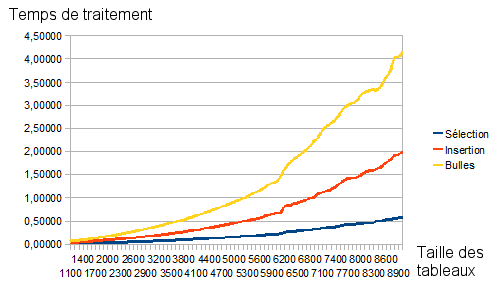
\includegraphics[scale=0.5]{tris_empiriques_grph.png}

\printbibliography

\end{document}